\documentclass[12pt,a4paper,twoside]{article}
\usepackage{labor}
\begin{document}

%fill for cover and header creation
\newcommand\laboratorynumber{2}
\title{Dünne Linsen}
\newcommand\supervisor{Ditlbacher, Harald}
\newcommand\groupnumber{42}

\newcommand\participantonelastname{Eisner}
\newcommand\participantonefirstname{Nico}
\newcommand\participantoneid{12214121}
\newcommand\participanttwolastname{Waldl}
\newcommand\participanttwofirstname{Philip}
\newcommand\participanttwoid{12214120}
\author{\participantonelastname \ \& \participanttwolastname}

\newcommand\degreeid{UB 033 678}
\newcommand\semester{23WS}
\date{17.11.2023}

%select correct course title
%\newcommand\coursetitle{Einführung in die \\ physikalischen Messmethoden}
%\newcommand\coursetitle{Laborübungen 1: \\ Mechanik und Wärme}
\newcommand\coursetitle{Laborübungen 2: \\ Elektrizität, Magnetismus, Optik}
%\newcommand\coursetitle{Fortgeschrittenen Praktikum 1: \\ Technische Physik}
%\newcommand\coursetitle{Fortgeschrittenen Praktikum 2: \\ Allgemeine Physik}

%\begin{titlepage}
   \begin{center}
       \begin{figure}[H]
            \begin{minipage}[h]{30mm}
                \centerline{
\includegraphics[height=15mm]{cover_nudes/tugraz.png}}
            \end{minipage}
            \hfill
            \begin{minipage}[h]{30mm}
                \centerline{
\includegraphics[height=15mm]{cover_nudes/nawi_graz.png}}
            \end{minipage}
            \hfill
            \begin{minipage}[h]{30mm}
                \centerline{
\includegraphics[height=15mm]{cover_nudes/uni-graz.png}}
            \end{minipage}
        \end{figure}
        
        \large{\emph{Institut für Experimentalphysik der Technischen Universität Graz \\
        \& Institut für Physik der Universität Graz}} \\
        \vspace{5mm}
        
        {\Huge \textbf{\coursetitle}}
        \vspace{5mm}
        
        {\huge \laboratorynumber: \thetitle}
    \end{center}
    
    \vfill
    
    \begin{table}[H]
        \LARGE
        \centering
        \begin{tabular}{r l}
            Betreuer:       & \supervisor \\
            Gruppennummer:  & \groupnumber \\
            \\
            Name:           & \participantonelastname, \participantonefirstname \\
            Matrikelnummer: & \participantoneid \\
            Name:           & \participanttwolastname, \participanttwofirstname \\
            Matrikelnummer: & \participanttwoid \\
            \\
            Kennzahl:       & \degreeid \\
            Datum:          & \semester \ | \thedate
        \end{tabular}
    \end{table}
    \vspace{4cm}
\end{titlepage}
\clearpage
\setcounter{page}{1}

%\maketitle %short title alternative

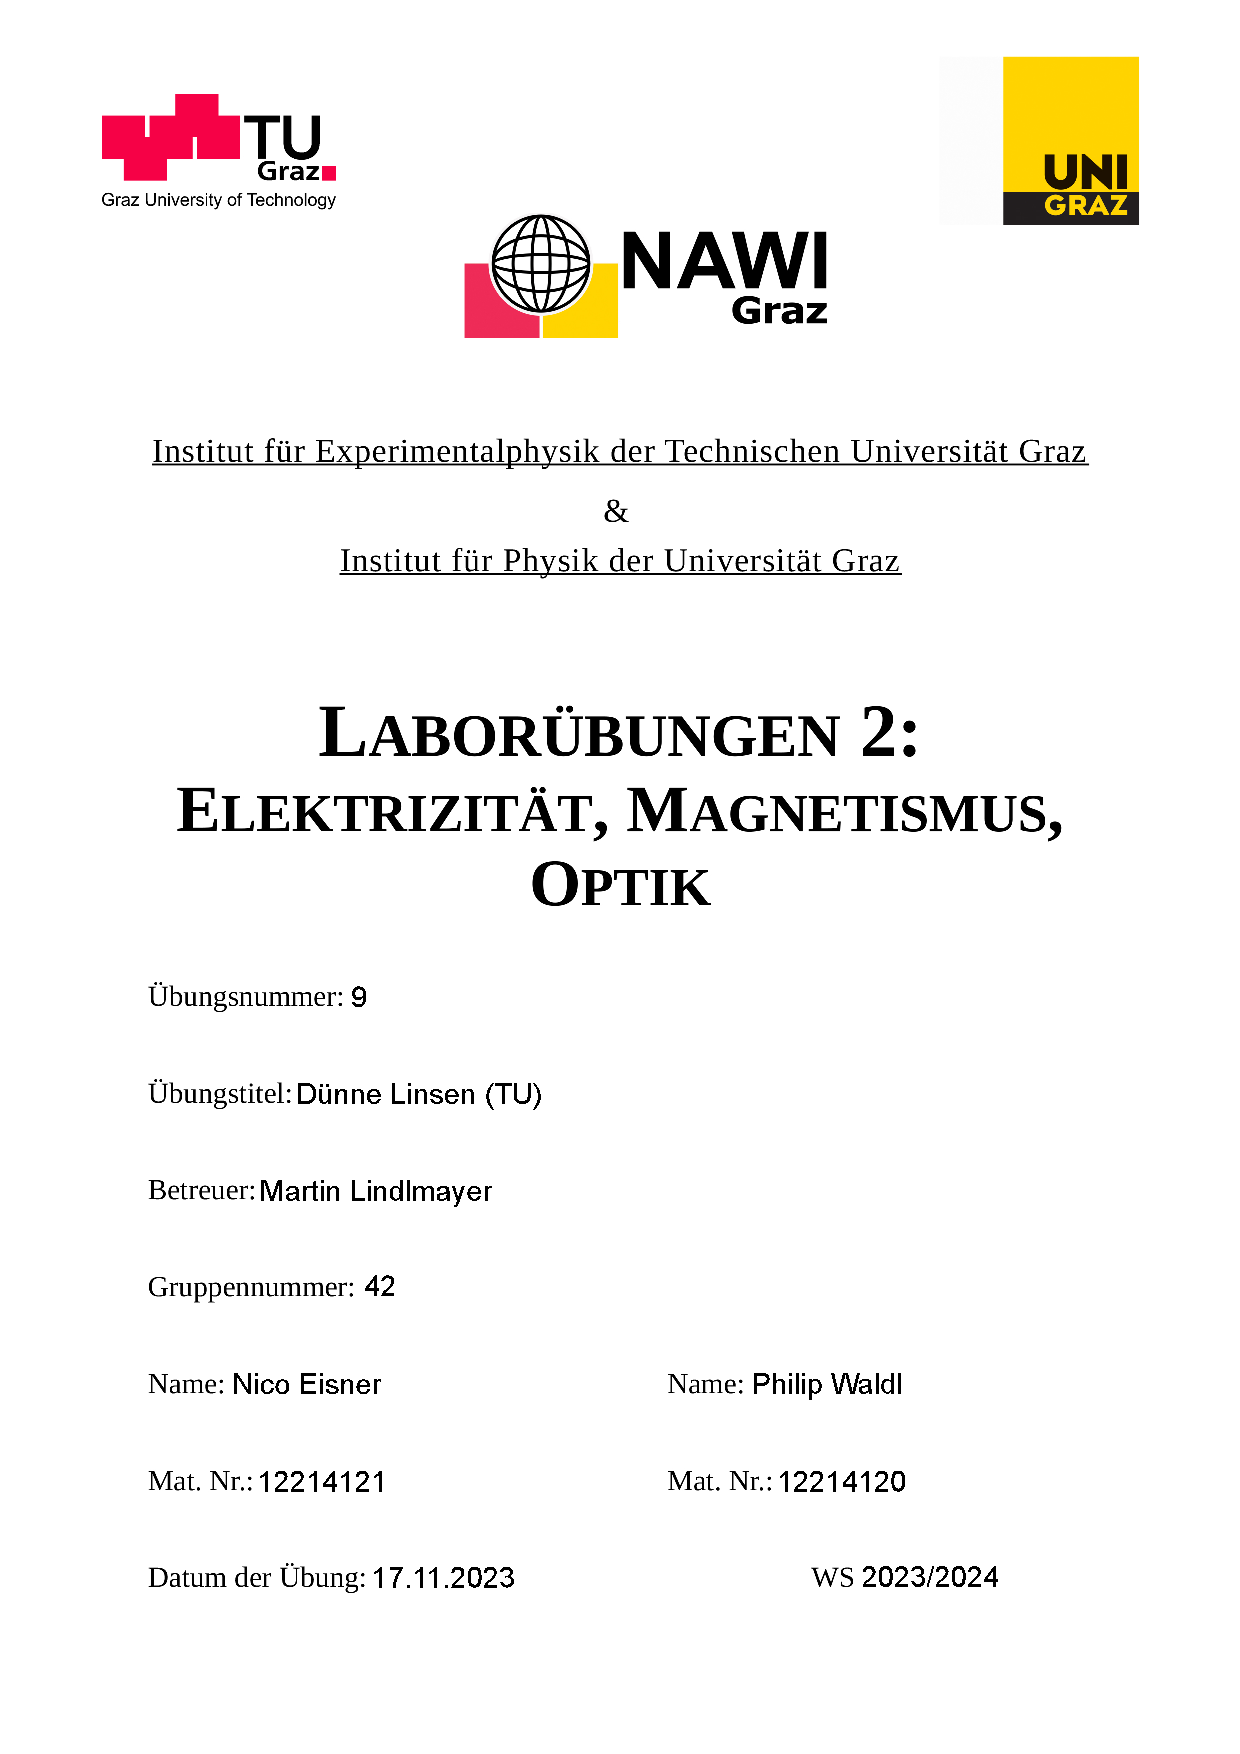
\includepdf[pages={1}]{../Deckblätter/Deckblatt_Dünne_Linsen.pdf}

\tableofcontents
\newpage

\section{Aufgabenstellung} %jo beschreibn wos gmocht host ------------------------------
Im Experiment Dünne Linsen gilt es Brennweite einer Sammellinse über zwei verschiedene Metoden zu bestimmen. 
Die Erste Methode ist jene nach der Laplace'sche Methode, die zweite nach dem Bessel'schen Verfahren. 
Desweiteren ist die Brennweite einer Zerstreuungslinse zu bestimmen. 
Zum schluss sollen noch einige Linsenfehler veranschaulicht werden. 
\\
\\
Gesuche Größen: 
\begin{itemize}
    \item Brennweite Laplace Sammellinse
    \item Brennweite Bessel Sammellinse
    \item Brennweite Zerstreuungslinse
\end{itemize}

\noindent
Alle Informationen und Methodiken wurden uns von der Technischen Universität bereitgestellt \cite{teachcenter2}. 

\section{Voraussetzungen \& Grundlagen} %Grundlagen erklären, Formeln mit erklärung
Für die Bestimmung der Brennweite einer Sammellinse gibt es, wie im vorherigen Kapitel erwähnt, mehrere Verfahren. 
\\
\\
Bei der Laplace'sche Methode Methode wird durch Messung der Längen $g$ und $b$ bei fokussierten Bild die Brennweite $f$ bestimmt. 
In der folgenden Abbildung \ref{fig:laplace_theorie} sieht man die Längen dargestellt. Dabei ist die Bildweite $b$ jene zwischen Linse und Schirm und die Gegenstandweite $g$ jene zwischen Projektor und Linse. 

\begin{figure}[H]
    \centering
    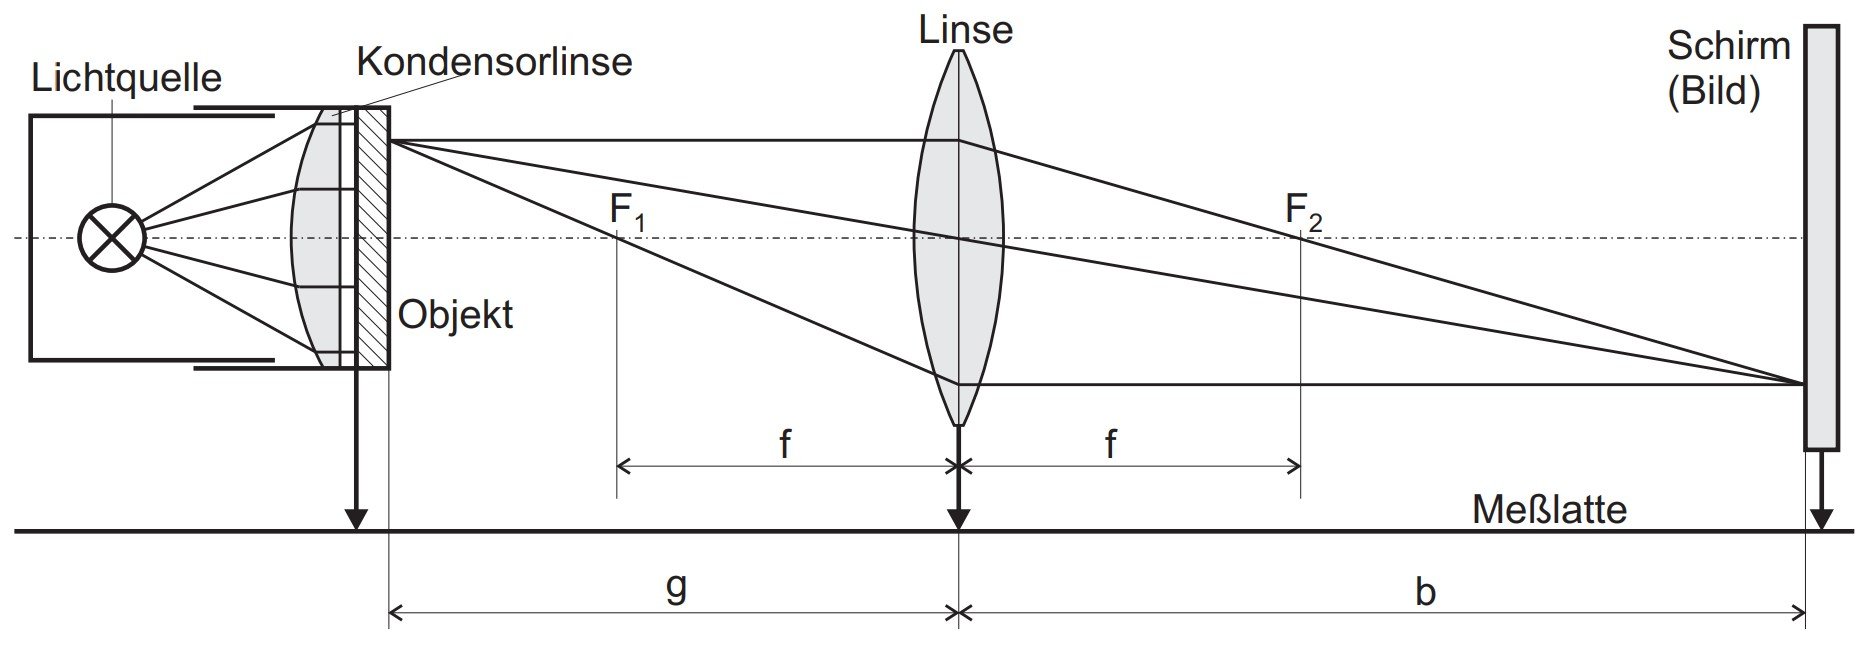
\includegraphics[width=0.6\linewidth]{nudes/laplace_theorie.jpg}
    \caption{Theoretischer Aufbau der Laplace'schen Methode. Bild aus Skriptum Dünne Linsen Seite 2 entnommen \cite{teachcenter2}. }
    \label{fig:laplace_theorie}
\end{figure}

\noindent
Mit der Formel \ref{eq:laplace} lässt sich aus der Bildweite $b$ und der Gegenstandweite $g$ die Brennweite $f$ wie deren Unsicherheit $\Delta f$ berrechnen. 

\begin{equation}
    \label{eq:laplace}
    \centerline{$\frac{1}{f}=\frac{1}{g} + \frac{1}{b}$ \\ $\Delta f = \vert \frac{\partial f}{\partial g} * \Delta g \vert + \vert \frac{\partial f}{\partial b} * \Delta b \vert$}
\end{equation}

\noindent
Ähnlich sieht es bei dem Bessel'schen Verfahren aus. Das Bild wird fokussiert. Durch bestimmung der Bildweite $b$ und der Gegenstandweite $g$ lässt sich der Gesamtabstand $a = g+b$ berrechnen. 
Die Linse wird verschoben, bis das Bild erneut scharf zu erkennen ist. Diese Strecke ist die Verschiebung $e$ wie in Abbildung \ref{fig:bessel_theorie} zu erkennen ist.  

\begin{figure}[H]
    \centering
    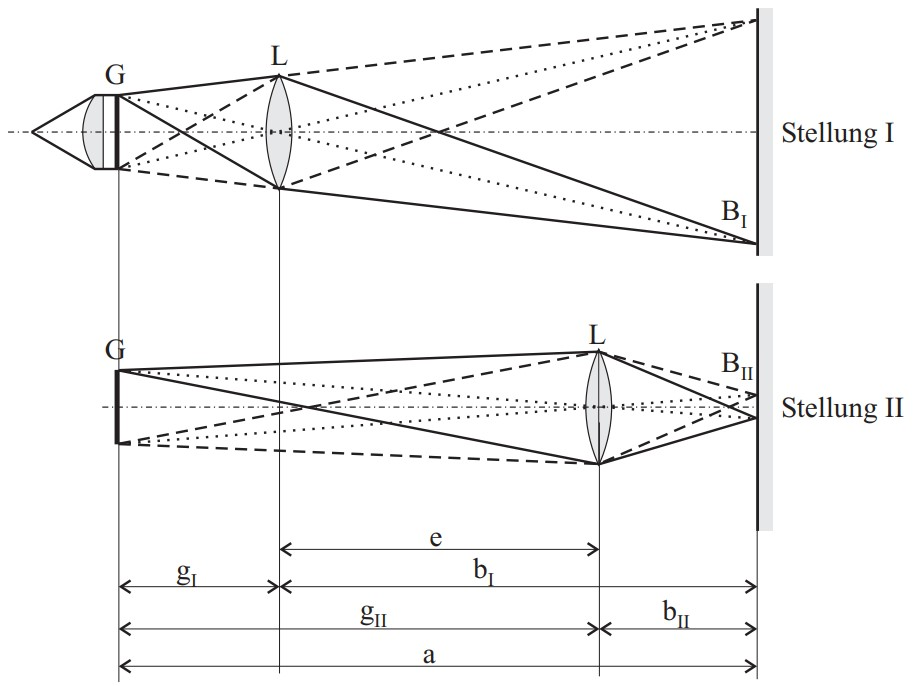
\includegraphics[width=0.6\linewidth]{nudes/bessel_theorie.jpg}
    \caption{Theoretischer Aufbau des Bessel'schen Verfahrens. Bild aus Skriptum Dünne Linsen Seite 3 entnommen \cite{teachcenter2}. }
    \label{fig:bessel_theorie}
\end{figure}

\noindent
Durch die Formel \ref{eq:bessel} lässt sich die Brennweite $f$ sowie deren Unsicherheit $\Delta f$ berrechnen. 

\begin{equation}
    \label{eq:bessel}
    \centerline{$f=\frac{1}{4} (\frac{a^2 - e^2}{a})$ \\ $\Delta f = \vert \frac{\partial f}{\partial a} * \Delta a \vert + \vert \frac{\partial f}{\partial e} * \Delta e \vert$}
\end{equation}

\noindent
Um die Brennweite $f_s$ einer Zerstreuungslinse zu bestimmen benötigt man die Gegenstandweite $g'$ sowie die Bildweite $b$. 
Um diese zu bestimmen, wird die Linse in einer Gegenstandweite $g'$ zum Schirm aufgestellt. Durch Verschieben des Schirmes, bis das Bild scharf zu erkennen ist wird die Bildweite $b$ bestimmt. Die Brennweite $f_s$ wird mit folgender Formel bestimmt. 

\begin{equation}
    \label{eq:Zerstreuungslinse}
    \centerline{$\frac{1}{f_s}=\frac{1}{g'} + \frac{1}{b}$ \\ $\Delta f_s = \vert \frac{\partial f_s}{\partial g'} * \Delta g' \vert + \vert \frac{\partial f_s}{\partial b} * \Delta b \vert$}
\end{equation}

\noindent
Hierbei ist jedoch anzumerken, dass die Brennweite $f_s$ ein negativer Wert ist. 
\\
\\
Ein wichtiger Punkt ist, dass bei den Formeln \ref{eq:laplace} und \ref{eq:Zerstreuungslinse} nicht die Brennweite $f$ berrechnet wird, sondern 1/$f$. Dieser Wert entspricht den Dioptrien $D$. Daher ist es wichtig den Kehrwert der Dioptrien $D$ zu bilden um die Brennweite $f$ zu erhalten. 

\begin{equation}
    \label{eq:Dioptirn}
    \centerline{$D = \frac{1}{f}=> f = \frac{1}{D}$}
\end{equation}

\noindent
Da in diesem Versuch mehrere Messdaten aufgenommen werden, kommt es zu mehreren Brennweiten $f$ bei der Berrechnung. Um einen Wert zu erhalten ist es wichtig, den Mittelwert sowie die Standardabweichung zu berrechnen. 
\\
Für die berechnung des Mittelwertes $\bar{f}$, benötigt man die Anzahl N sowie die einzelnen Brennweiten $f$. 

\begin{equation}
    \label{eq:Mittelwert}
    \centerline{$\bar{f} = \frac{1}{N} \sum_{i = 1}^{N} f_i $} 
\end{equation}

\noindent
Mit dem nun bekannten Mittelwert $\bar{f}$ lässt sich die Standardabweichung $\sigma_{f}$ berechnen. 

\begin{equation}
    \label{eq:Standardabweichung}
    \centerline{$\sigma_{f} = \sqrt{\frac{1}{N-1} \sum_{i = 1}^{N} (f_i - \bar{f})^2}$} 
\end{equation}

\section{Versuchsanordnung} %mit skizze kurz beschreiben ------------------------------
Die Versuche werden wie in den folgenden Bildern aufgebaut. Die Optischen Elemente befindet sich dabei auf einer Schiene, welche mit einem Lineal versehen ist. 


    \begin{figure}[H]
        \centering
        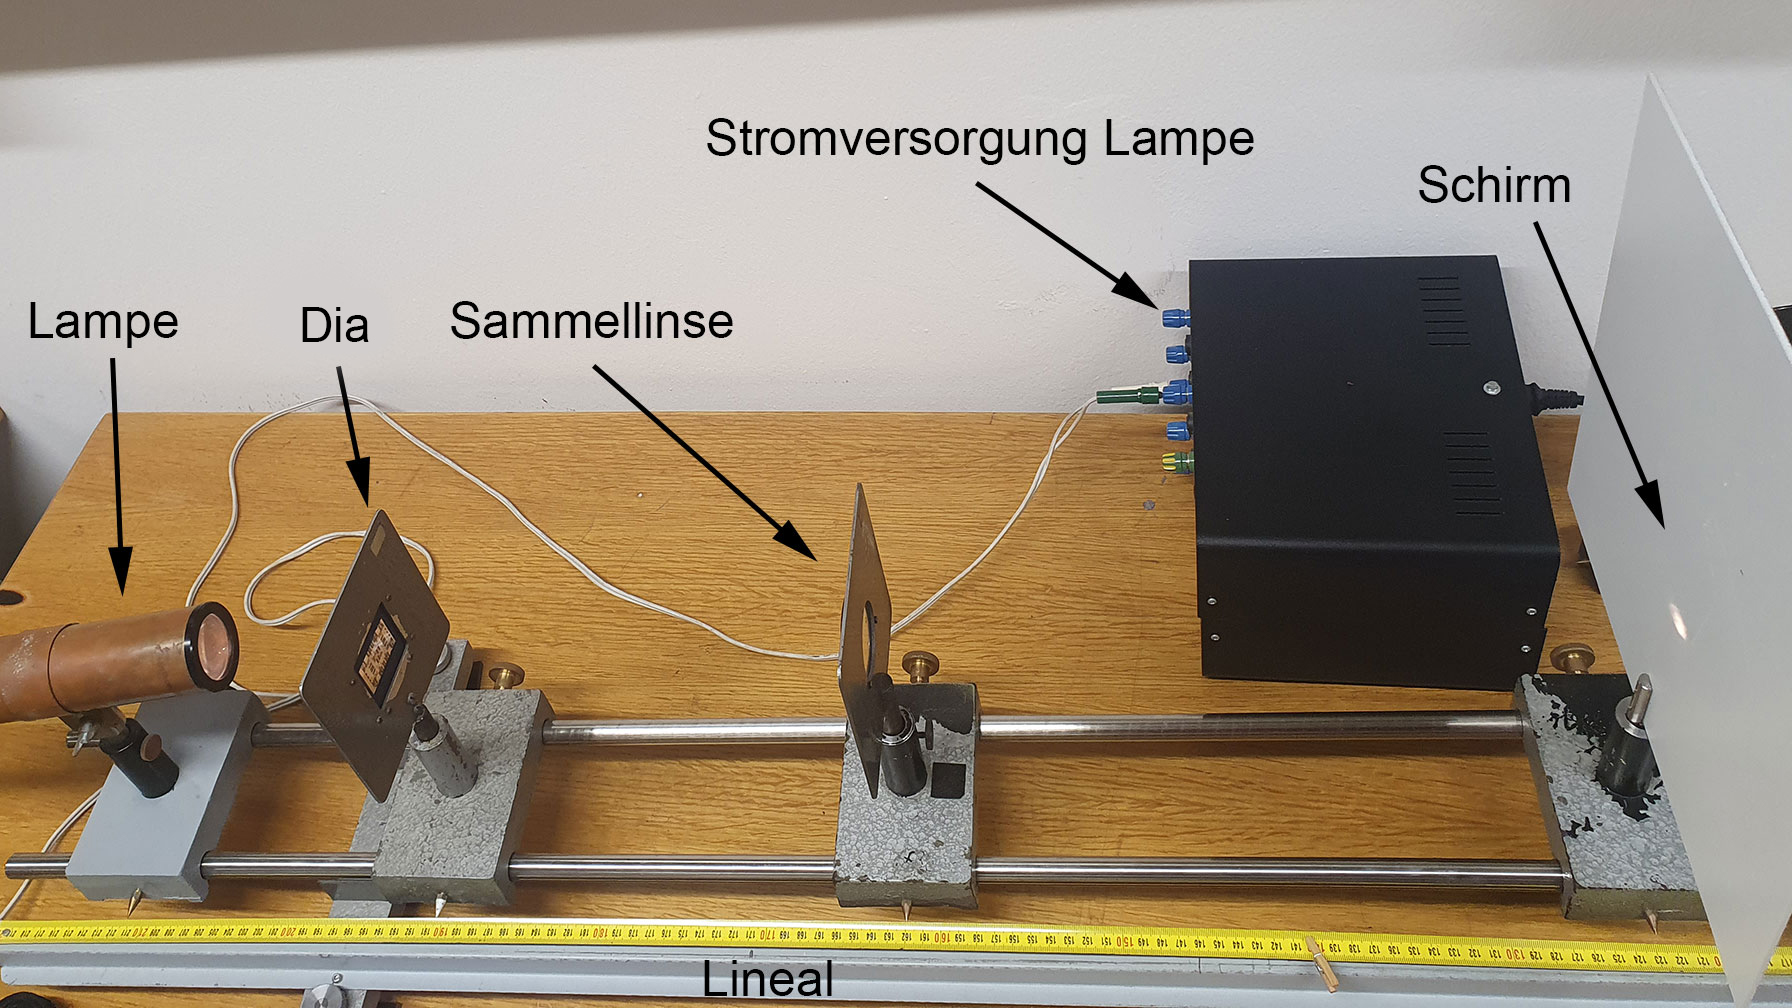
\includegraphics[width=0.6\linewidth]{nudes/komprimert/aufbau sammellinse.jpg}
        \caption{Aufbau der Versuche zur Bestimmung der Brennweite mit der Sammellinse. Beide Aufbauten sehen gleich aus. }
        \label{fig:aufbau Sammellinse}
    \end{figure}

    \begin{figure}[H]
        \centering
        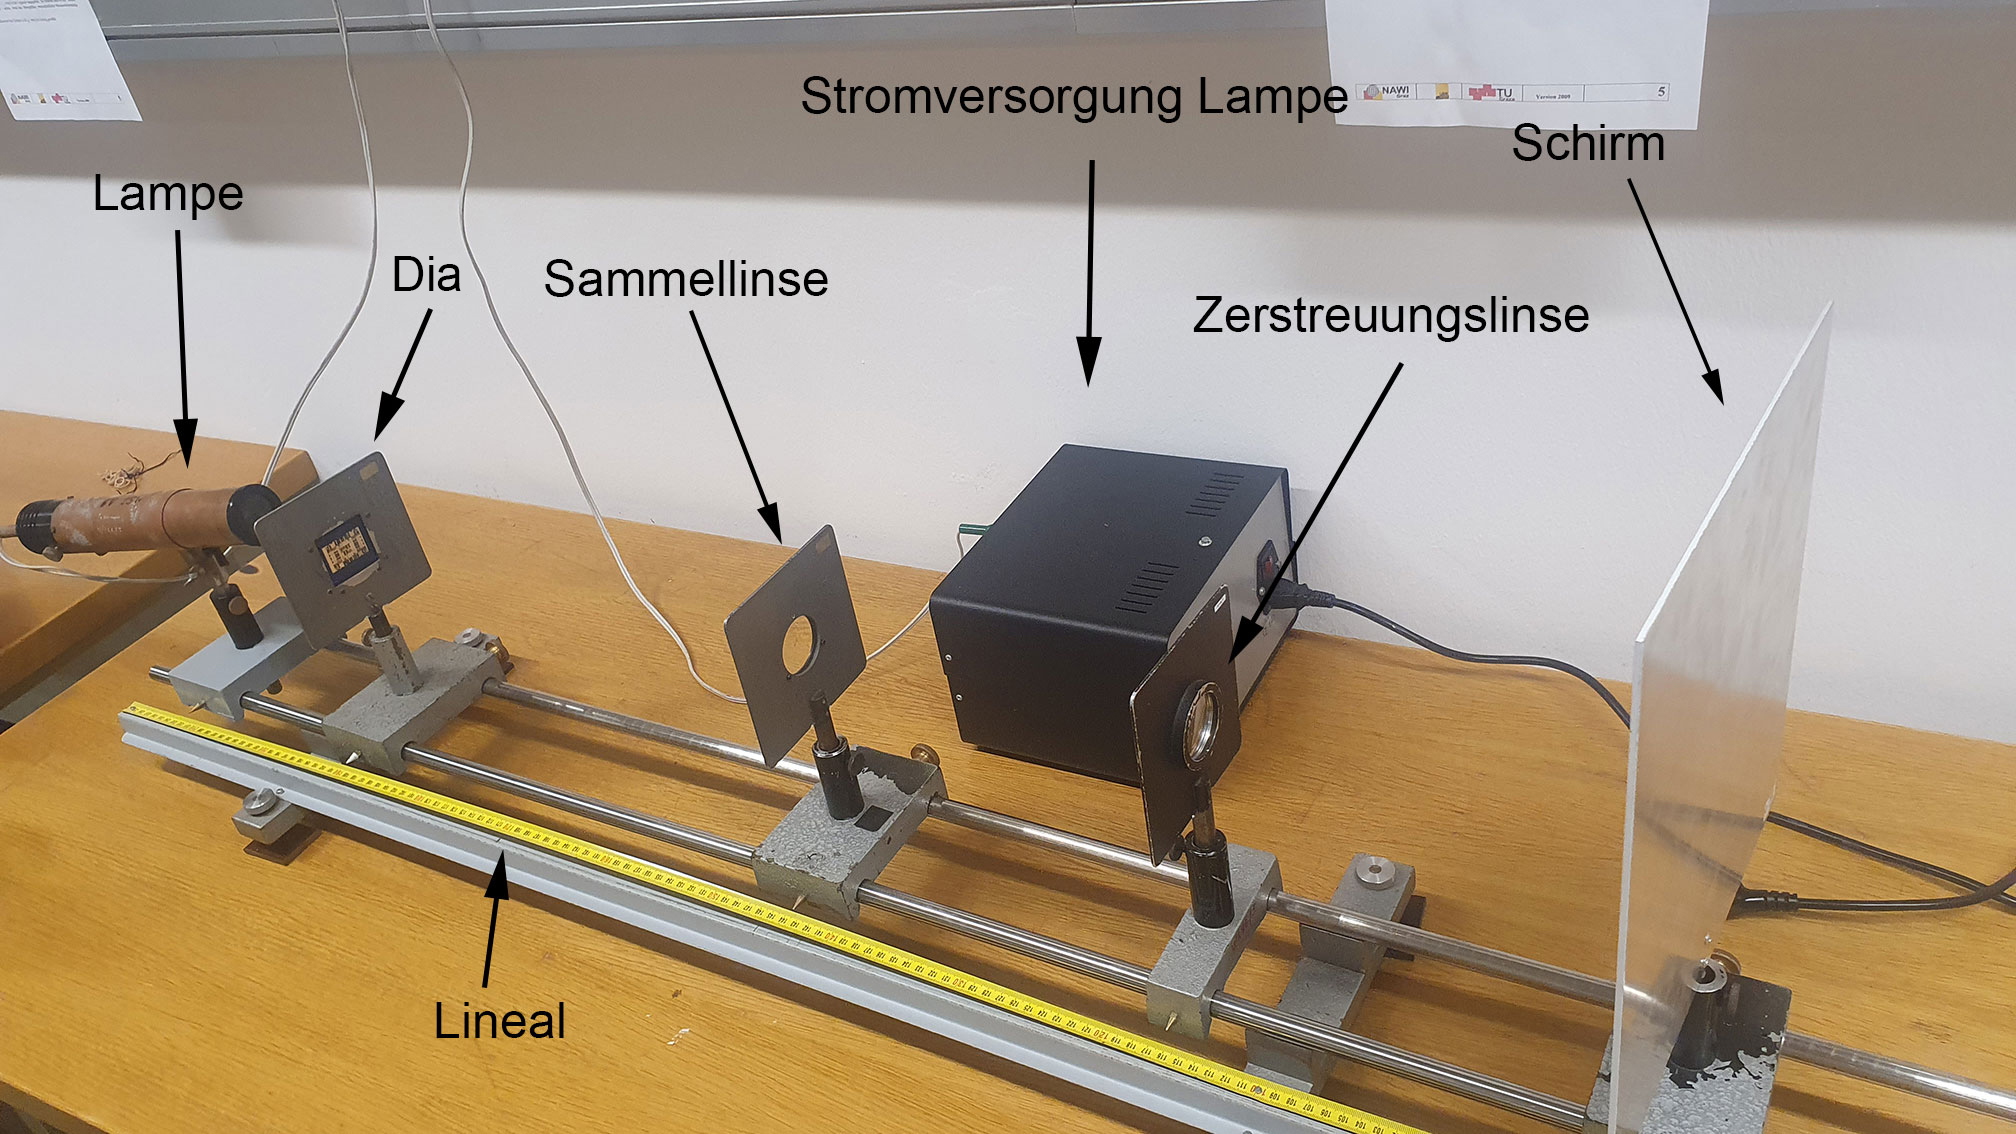
\includegraphics[width=0.6\linewidth]{nudes/komprimert/aufbau zerstreuungslinse.jpg}
        \caption{Versuchsaufbau für die Bestimmung der Brennweite der Zerstreuungslinse}
        \label{fig:aufbau Zerstreuungslinse}
    \end{figure}

    \begin{figure}[H]
        \centering
        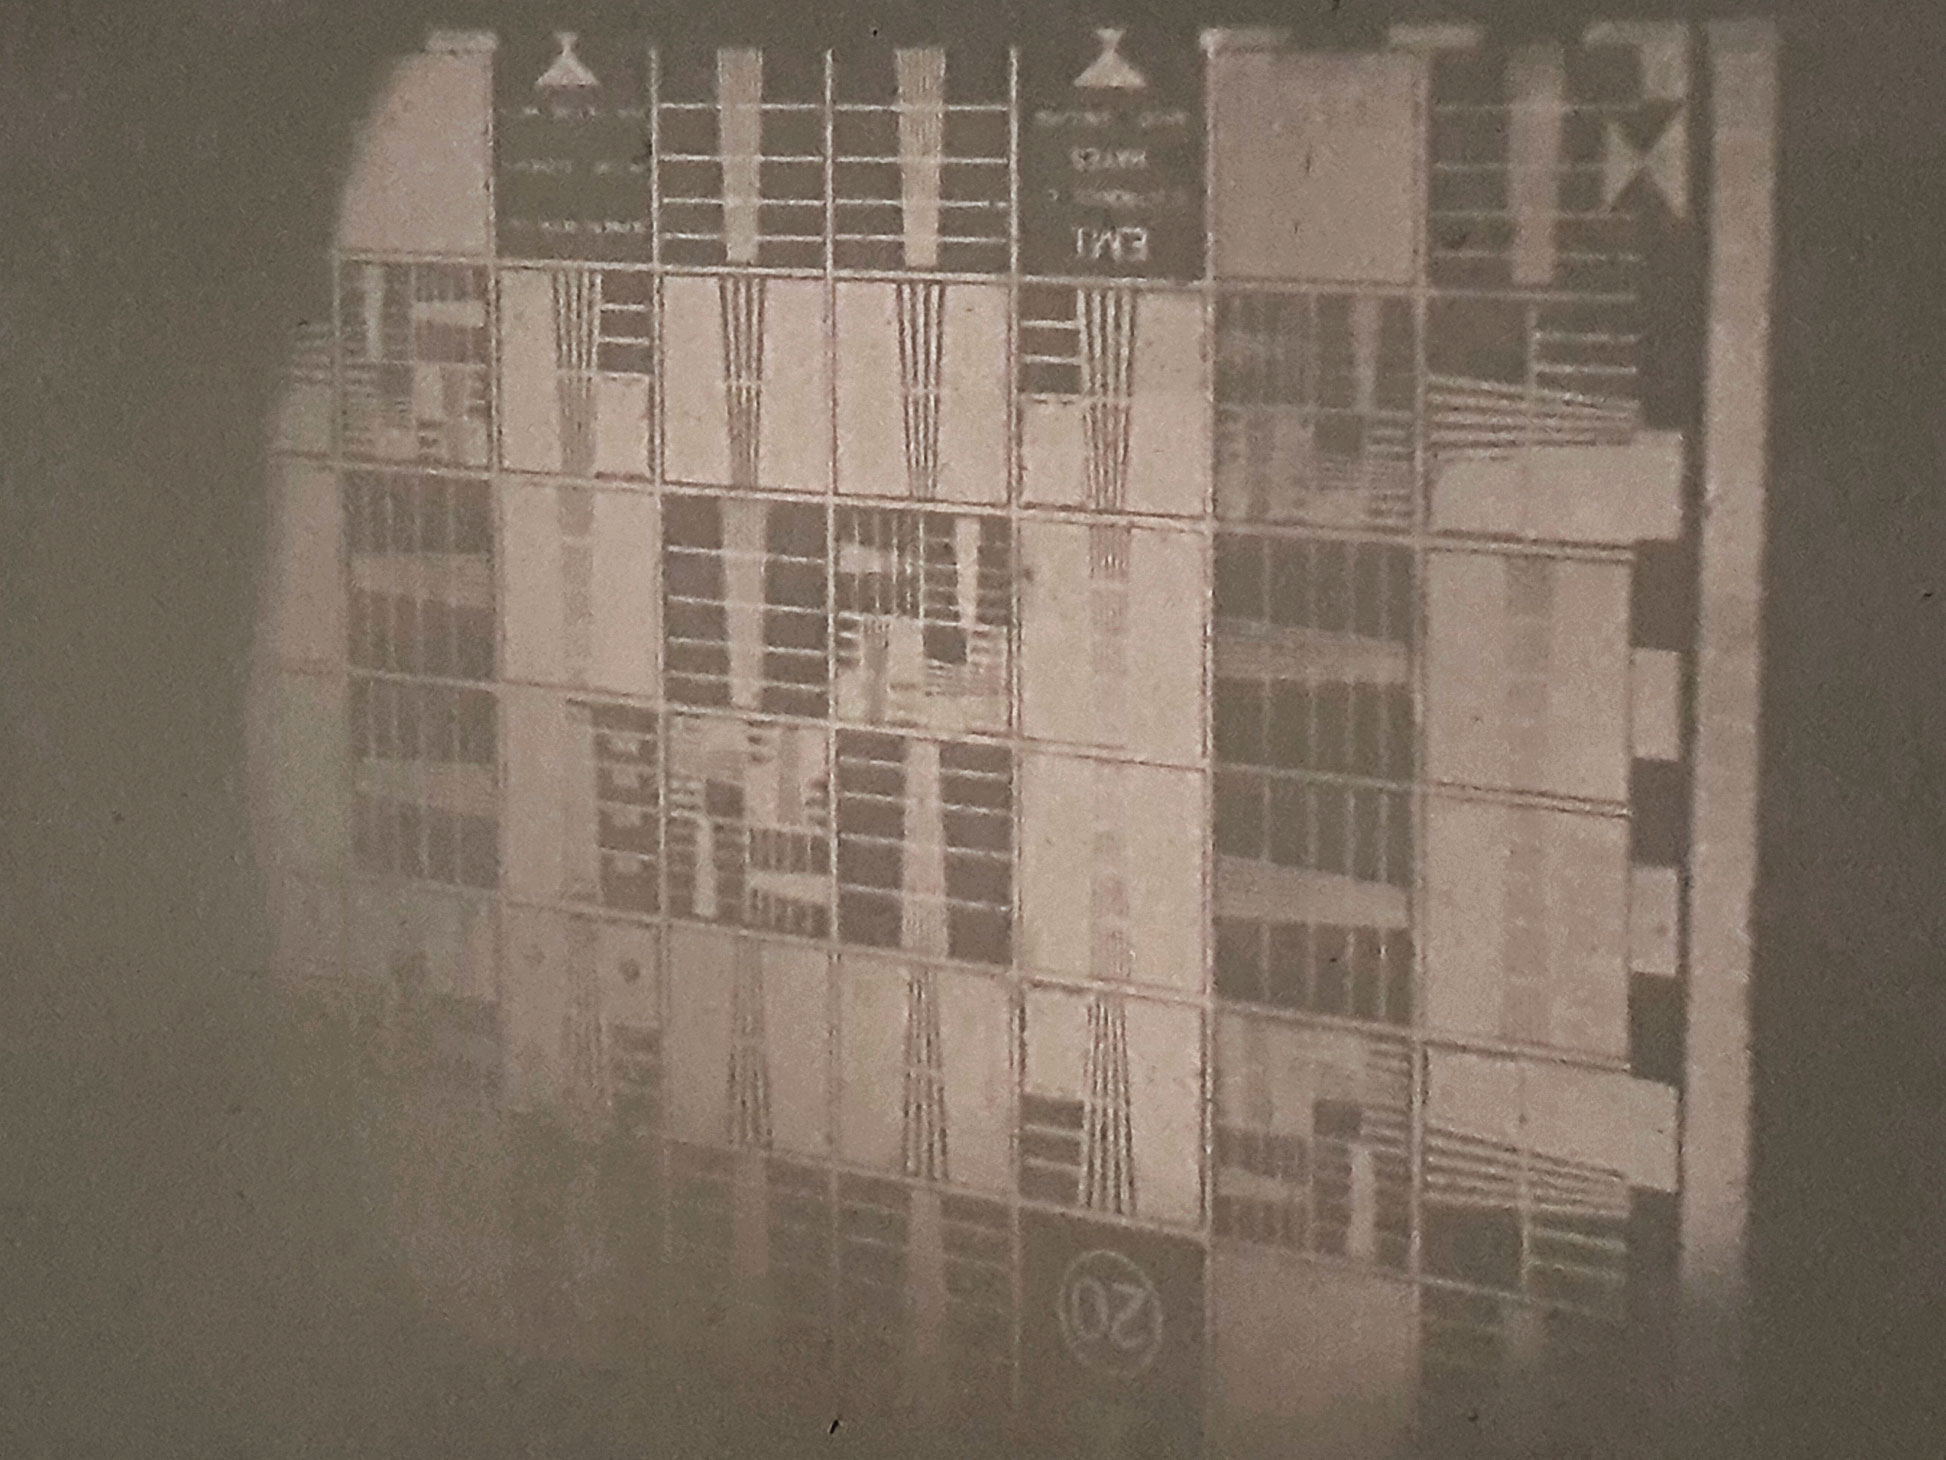
\includegraphics[width=0.6\linewidth]{nudes/komprimert/bild.jpg}
        \caption{Projeziertes, scharfgestelltes Bild}
        \label{fig:aufbau Bild}
    \end{figure}

\section{Geräteliste} %jo holt a listn ------------------------------

    \begin{table}[H]
        \centering
        \caption{Im Versuch verwendete Geräte und Utensilien.}
        \label{tab:geraete}
        \begin{tabular}{| l | l | l |}
            \hline
            Gerät  & Gerätenummer  & Unsicherheit \\
            \hline
            Lampe & {n.a} & {n.a} \\
            Sammellinse & {n.a} & {n.a} \\
            Zerstreuungslinse & {n.a} & {n.a} \\
            Schirm & {n.a} & {n.a} \\
            Lineal & {n.a} & $\pm 1.0 mm$ \\
        \end{tabular}
    \end{table}


\section{Versuchsdurchführung \& Messergebnisse} %nachvollziehbar und klar dargestellt ------------------------------
Um für den ersten Versuchsteil nach der Laplace'schen Methode die Gegenstandweite $g$ sowie die Bildweite $b$ zu bestimmen, werden insgesamt 10 Messversuche aufgestellt. 
Um diese zu bestimmen, wird mit dem auf der Schiene angebrachtem Lineal die Abstände von Linse zu Schirm ($b$) und Linse zu Lampe ($g$) gemessen. 
Der Schirm wird dabei jeweils um 10 cm verschoben. Die Linse wird so Verschoben, dass das Bild auf dem Schirm scharf abgebildet wird. Die Lampe hat dabei immer die gleiche Position. 

\begin{table}[H]
    \centering
    \caption{Messergebnisse der Abstände nach der Laplace'schen Methode für die Sammellinse. }
    \label{tab:messergebnisse Laplace}
    \begin{tabular}{| l | l | l | l |}
        \hline
        Nr.  & Schirm $\pm 0.1 $/ cm & Linse $\pm 0.1 $ / cm & Lampe $\pm 0.1 $ / cm \\
        \hline
        1  & 10.0   & 159.8  & 190.0 \\
        2  & 20.0   & 158.9  & 190.0 \\
        3  & 30.0   & 158.4  & 190.0 \\
        4  & 40.0   & 157.8  & 190.0 \\
        5  & 50.0   & 156.9  & 190.0 \\
        6  & 60.0   & 155.9  & 190.0 \\
        7  & 70.0   & 154.1  & 190.0 \\
        8  & 80.0   & 151.4  & 190.0 \\
        9  & 90.0   & 143.6  & 190.0 \\
        10 & 100.0  & 141.2  & 190.0 \\
        \hline
    \end{tabular}
\end{table}

\noindent
Im zweiten Teil wird nach dem Bessel'schen Verfahren die Brennweite $f$ bestimmt. 
Der Versuch wird insgesamt 5 mal wiederholt. Der Schirm wird immer um 10 cm verschoben, die Lampe hat immer die gleiche Positon. Aus deren differenz lässt sich auch der Gesamtabstand $a$ bestimmen. 
Die Linse wird so eingestellt, dass das Bild auf dem Schirm scharf abgebildet wird. Anschließend verschiebt man die Linse soweit zum Schirm, bis das Bild erneut scharf abgebildet wird. Diese Strecke ist die Verschiebung $e$. 

\begin{table}[H]
    \centering
    \caption{Messergebnisse der Abstände nach dem Bessel'schen Verfahren für die Sammellinse. Zu beachten ist, dass Pos 1 und Pos 2 die Positionen der Linse representieren. }
    \label{tab:messergebnisse Bessel}
    \begin{tabular}{| l | l | l | l | l |}
        \hline
        Nr.  & Schirm $\pm 0.1 $ / cm &  Pos. 1 $\pm 0.1 $ / cm & Pos. 2 $\pm 0.1 $ / cm & Lampe $\pm 0.1 $ / cm \\
        \hline
        1  & 30.0   & 158.5 & 61.1  & 190.0 \\
        2  & 40.0   & 158.0 & 70.9  & 190.0 \\
        3  & 50.0   & 157.3 & 81.7  & 190.0 \\
        4  & 60.0   & 155.9 & 92.8  & 190.0 \\
        5  & 70.0   & 154.5 & 104.4 & 190.0 \\
        \hline
    \end{tabular}
\end{table}

\noindent
Im dritten Teil, bei der Zerstreuungslinse, wird die Zerstreuungslinse auf einen Abstand gestellt. In einen beliebigen Abstand wird der Schirm aufgestellt. 
Die differenz dieser Abstände ist die Gegenstandweite $g'$. Nun wird der Schirm soweit entfernt, bis das Bild scharf zu erkennen ist. 
Die differenz zu der ersten Position des Schirmes ist die Bildweite $b$. 

\begin{table}[H]
    \centering
    \caption{Messergebnisse der Abstände für die Zerstreuungslinse. Zu beachten ist, dass Pos 1 und Pos 2 die Positionen des Schirmes representieren. }
    \label{tab:messergebnisse Zerstreuungslinse}
    \begin{tabular}{| l | l | l | l |}
        \hline
        Nr.  & Linse $\pm 0.1 $/ cm & Pos. 1 $\pm 0.1 $ / cm & Pos. 2 $\pm 0.1 $ / cm \\
        \hline
        1  & 50.0   & 40.0 & 34.0 \\
        2  & 60.0   & 50.0 & 43.6 \\
        3  & 65.0   & 55.0 & 48.6 \\
        4  & 32.0   & 20.0 & 9.0  \\
        5  & 45.0   & 30.0 & 9.0  \\
        6  & 64.0   & 50.0 & 33.0 \\
        7  & 85.0   & 70.0 & 48.0 \\
        8  & 90.0   & 80.0 & 73.5 \\
        9  & 100.0  & 85.0 & 62.0 \\
        10 & 81.0   & 70.0 & 62.0 \\
        \hline
    \end{tabular}
\end{table}

\noindent
Für den letzten Teil, welcher die Linsenfehler beinhaltet, versucht man einige Linsenfehler darzustellen. Durch leichtes drehen der Linse kann der Fehler der Verzerrung dargestellt werden. Über dem projeziertem Bild ist chromatische Aberration erkennbar. 

\section{Auswertung und Unsicherheitsanalyse} %Nicht nur zahlen angeben ------------------------------

In der Auswertung werden zur erhöhten Genauigkeit durchgehend ungerundete Werte bis zu den Endergebnissen verwendet und nur zur Darstellung gerundet. \\
Zur Berechnung der Unsicherheiten wird, wenn nicht anders angegeben, die Größtunsicherheitsmethode verwendet.
\\
\\
Aus den Messdaten der Tabelle \ref{tab:messergebnisse Laplace} lassen sich nun die Gegenstandweite $g$ und die Bildweite $b$ berrechnen. 
Für die Bildweite $b$ subtrahiert man die Position der Linse mit der Position des Schirmes. Für die Gegenstandweite $g$ subtrahiert man die Position des Dias mit der Position der Linse. Die Unsicherheiten sind in diesen Fall gleich. 
\\
Setzt man diese Werte in die Formel \ref{eq:laplace} ein, so kommt man auf die Brennweite $f$. Hierbei ist jedoch anzumerken, dass man bei der Berrechnung von 1/g+1/b den Wert 1/f bekommt, was den Dioptrien $D$ entspricht. Um die Brennweite $f$ zu bekommen muss man den Kehrwert des Ergebnisses nehmen. 


\begin{table}[H]
    \centering
    \caption{Bildweite $b$ und Gegenstandweite $g$ aus den Messdaten der Tabelle \ref{tab:messergebnisse Laplace} sowie die daraus berrechnete Brennweite $f$. }
    \label{tab:berechnung Laplace}
    \begin{tabular}{| l | l | l | l |}
        \hline
        Nr.  & $b$ $\pm 0.1 $/ cm & $g$ $\pm 0.1 $ / cm & $f$ $\pm 0.1 $ / cm \\
        \hline
        1  & 149.8  & 30.2  &  25.2 \\% 25.14  $\pm$ 0.08   \\
        2  & 138.9  & 31.1  &  25.5 \\% 25.43  $\pm$ 0.08   \\
        3  & 128.4  & 31.6  &  25.4 \\% 25.36  $\pm$ 0.07   \\
        4  & 117.8  & 32.2  &  25.3 \\% 25.29  $\pm$ 0.07   \\
        5  & 106.9  & 33.1  &  25.3 \\% 25.28  $\pm$ 0.07   \\
        6  & 95.9   & 34.1  &  25.2 \\% 25.16  $\pm$ 0.07   \\
        7  & 84.1   & 35.9  &  25.2 \\% 25.16  $\pm$ 0.06   \\
        8  & 71.4   & 38.6  &  25.1 \\% 25.06  $\pm$ 0.06   \\
        9  & 53.6   & 46.4  &  24.9 \\% 24.88  $\pm$ 0.06   \\
        10 & 41.2   & 48.8  &  22.4 \\% 22.34  $\pm$ 0.06   \\
        \hline
    \end{tabular}
\end{table}

\noindent 
Aus den berrechneten Brennweiten $f$ wird der Mittelwert $\bar{f}$ und die Standardabweichung $\sigma_f$ mithilfe der Formeln \ref{eq:Mittelwert} und \ref{eq:Standardabweichung} gebildet. 
Somit kommt man auf den Mittelwert $\bar{f} = (24.9 \pm 0.1)cm$ mit Standardabweichung $\sigma_f = (1.0) cm$ für die Brennweiten $f$ nach dem Laplace'schen Verfahren. 
\\
\\
Eine weitere Möglichkeit die Dioptrien zu bestimmen, ist sie aus einen Diagramm mit den Kehrwerten der Gegenstandweite $g$ und Bildweite $b$ abzulesen. 

\begin{figure}[H]
    \centering
    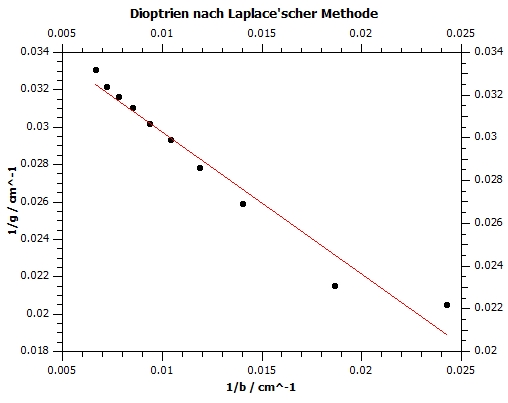
\includegraphics[width=0.6\linewidth]{nudes/dioptrin laplace.jpg}
    \caption{Dioptrien mit einer Steigung von $(-0.76 \pm 0.06) cm^{-1}$}
    \label{fig:Dioptrien laplace plot}
\end{figure}

\noindent
Für die Methode nach Bessel sieht es ähnlich aus. Die Werte des Gesamtabstandes $a$ sowie die Verschiebung $e$ werden aus den Messdaten der Tabelle \ref{tab:messergebnisse Bessel} berrechnet. Eingesetzt in die Formel \ref{eq:bessel} erhält man die Brennweite $f$. 

\begin{table}[H]
    \centering
    \caption{Gesamtabstand $a$ und Verschiebung $e$ aus den Messdaten der Tabelle \ref{tab:messergebnisse Bessel} sowie die daraus berrechnete Brennweite $f$. }
    \label{tab:berechnung Bessel}
    \begin{tabular}{| l | l | l | l |}
        \hline
        Nr.  & $a$ $\pm 0.1 $ / cm &  $e$ $\pm 0.1 $ / cm & $f$ $\pm 0.1 $ / cm  \\
        \hline
        1  & 160.0   & 97.4 &  25.2  \\
        2  & 150.0   & 87.1 &  24.9  \\
        3  & 140.0   & 75.6 &  24.8  \\
        4  & 130.0   & 63.1 &  24.9  \\
        5  & 120.0   & 50.1 &  24.8  \\
        \hline
    \end{tabular}
\end{table}

\noindent
Wie zuvor wird auch der Mittelwert $\bar{f}$ und die Standardabweichung $\sigma_f$ aus den Formeln \ref{eq:Mittelwert} und \ref{eq:Standardabweichung} berechnet. 
Man kommt auf den Wert von $\bar{f} = (24.9 \pm 0.1) cm$ und $\sigma_f =( 0.2) cm$. 
\\
\\
Im dritten Teil wird die Brennweite $f_s$ einer Zerstreuungslinse bestimmt. Aus den Messergebnissen der Tabelle \ref{tab:messergebnisse Zerstreuungslinse} folgen die Werte der Gegenstandweite $g'$ und Bildweite $b$. 
Die Gegenstandweite $g'$ ist dabei die differenz von Pos. 1 und Linse, und die Bildweite $b$ ist die differenz von Linse und Pos. 2. 
Die Brennweite $f_s$ wird mithilfe der Formel \ref{eq:Zerstreuungslinse} unter berücksichtigung der Formel \ref{eq:Dioptirn} berechnet. 

\begin{table}[H]
    \centering
    \caption{Gegenstandweite $g'$ und Bildweite $b$ einer Zerstreuungslinse mit berechneter Brennweite $f_s$. }
    \label{tab:berechnung Zerstreuungslinse}
    \begin{tabular}{| l | l | l | l |}
        \hline
        Nr.  & $g'$ $\pm 0.1 $/ cm & $b$ $\pm 0.1 $ / cm & $f_s$ $\pm 0.1 $ / cm \\
        \hline
        1  & -10.0  & 16.0 & -26.7  \\
        2  & -10.0  & 16.4 & -25.7  \\
        3  & -10.0  & 16.4 & -25.7  \\
        4  & -12.0  & 23.0 & -25.1  \\
        5  & -15.0  & 36.0 & -25.8  \\
        6  & -14.0  & 31.0 & -25.6  \\
        7  & -15.0  & 37.0 & -25.3  \\
        8  & -10.0  & 16.5 & -25.4  \\
        9  & -15.0  & 38.0 & -24.8  \\
        10 & -11.0  & 19.0 & -26.2  \\
        \hline
    \end{tabular}
\end{table}

\noindent
Wie bei den vorherigen Teilen wird der Mittelwert $\bar{f_s}$ und die Standardabweichung $\sigma_{f_s}$ laut den Formeln \ref{eq:Mittelwert} und \ref{eq:Standardabweichung} berechnet. 
Man kommt auf das Ergebnis von $\bar{f_s} = (-25.6 \pm 0.1)cm$ und $\sigma_{f_s} = (0.6)cm$
\\
\\
Im letzten Teil gilt es einige Linsenfehler darzustellen. Wie in den Kapitel Messergebnisse beschrieben, wurde die Verzerrung sowie die chromatische Aberration dargestellt. 

\begin{figure}[H]
    \centering
    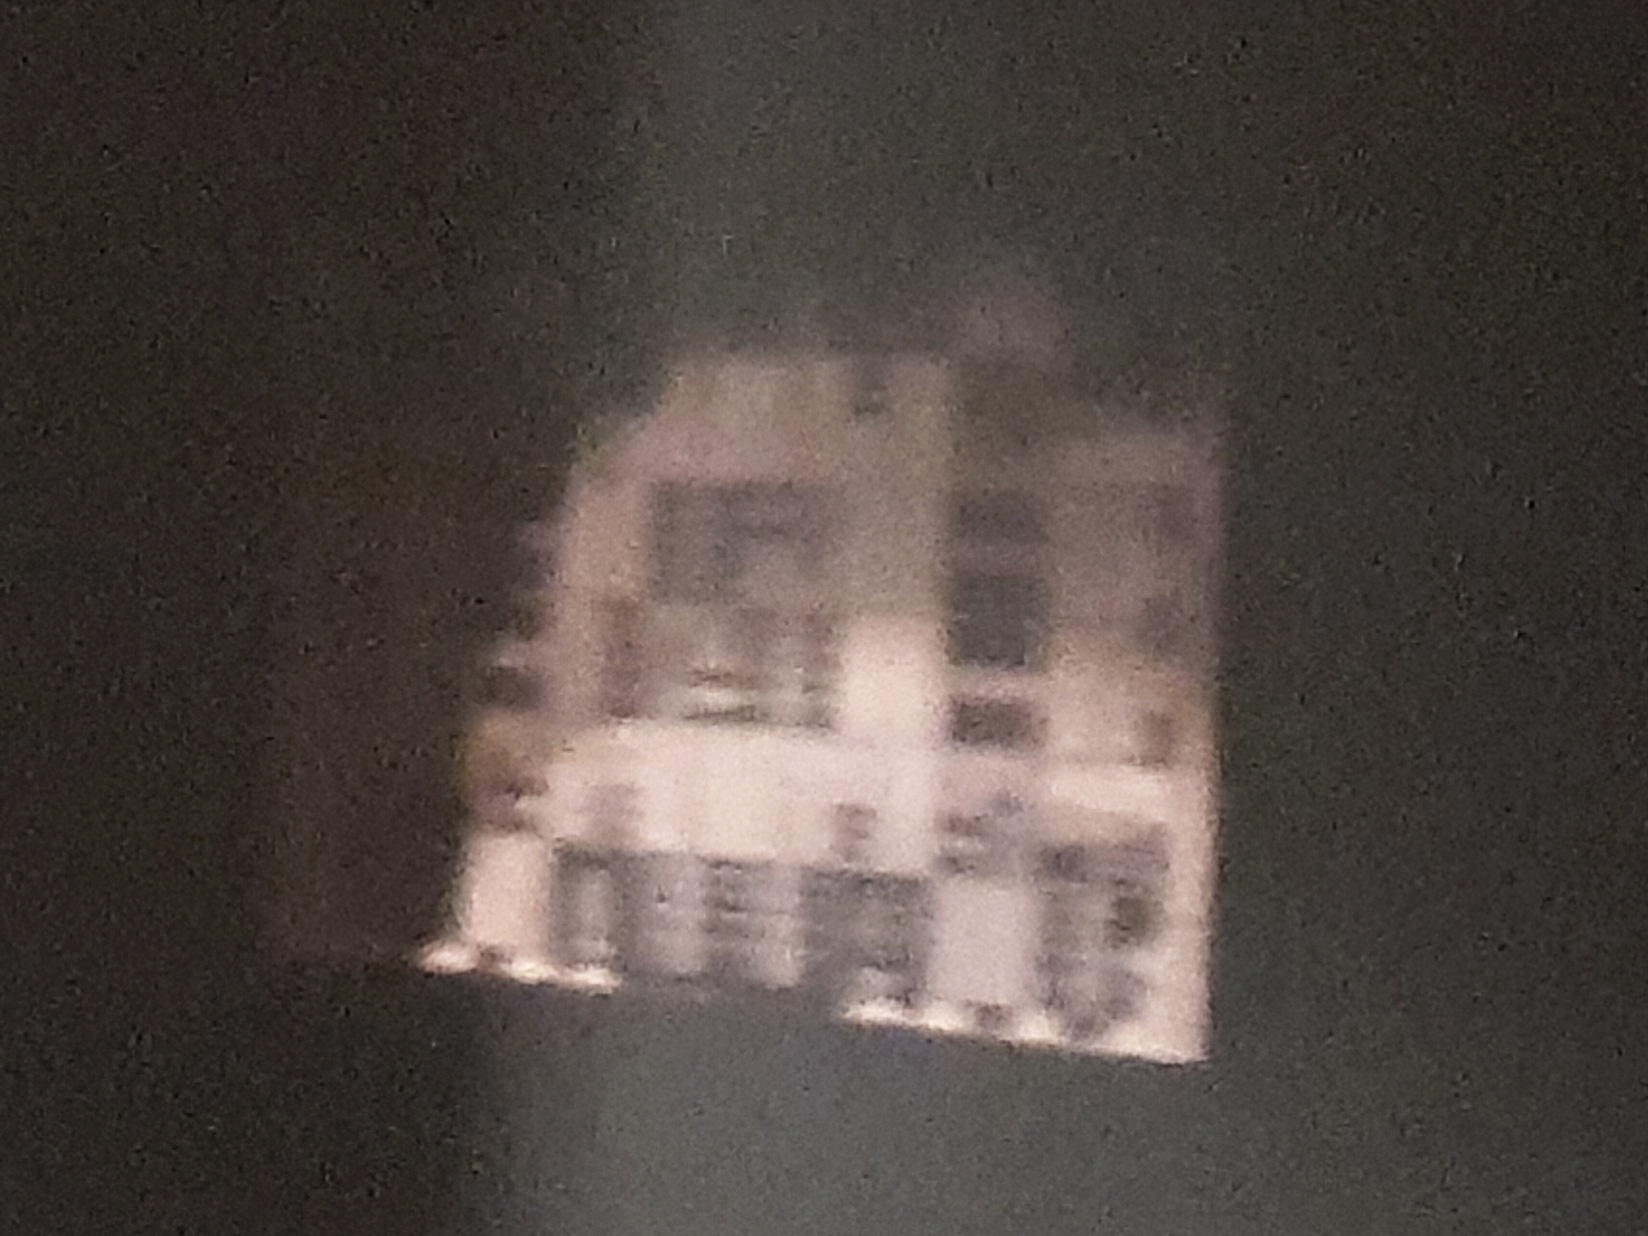
\includegraphics[width=0.6\linewidth]{nudes/komprimert/verzerrung.jpg}
    \caption{Verzerrung der Linse. }
    \label{fig:verzerrung}
\end{figure}

\begin{figure}[H]
    \centering
    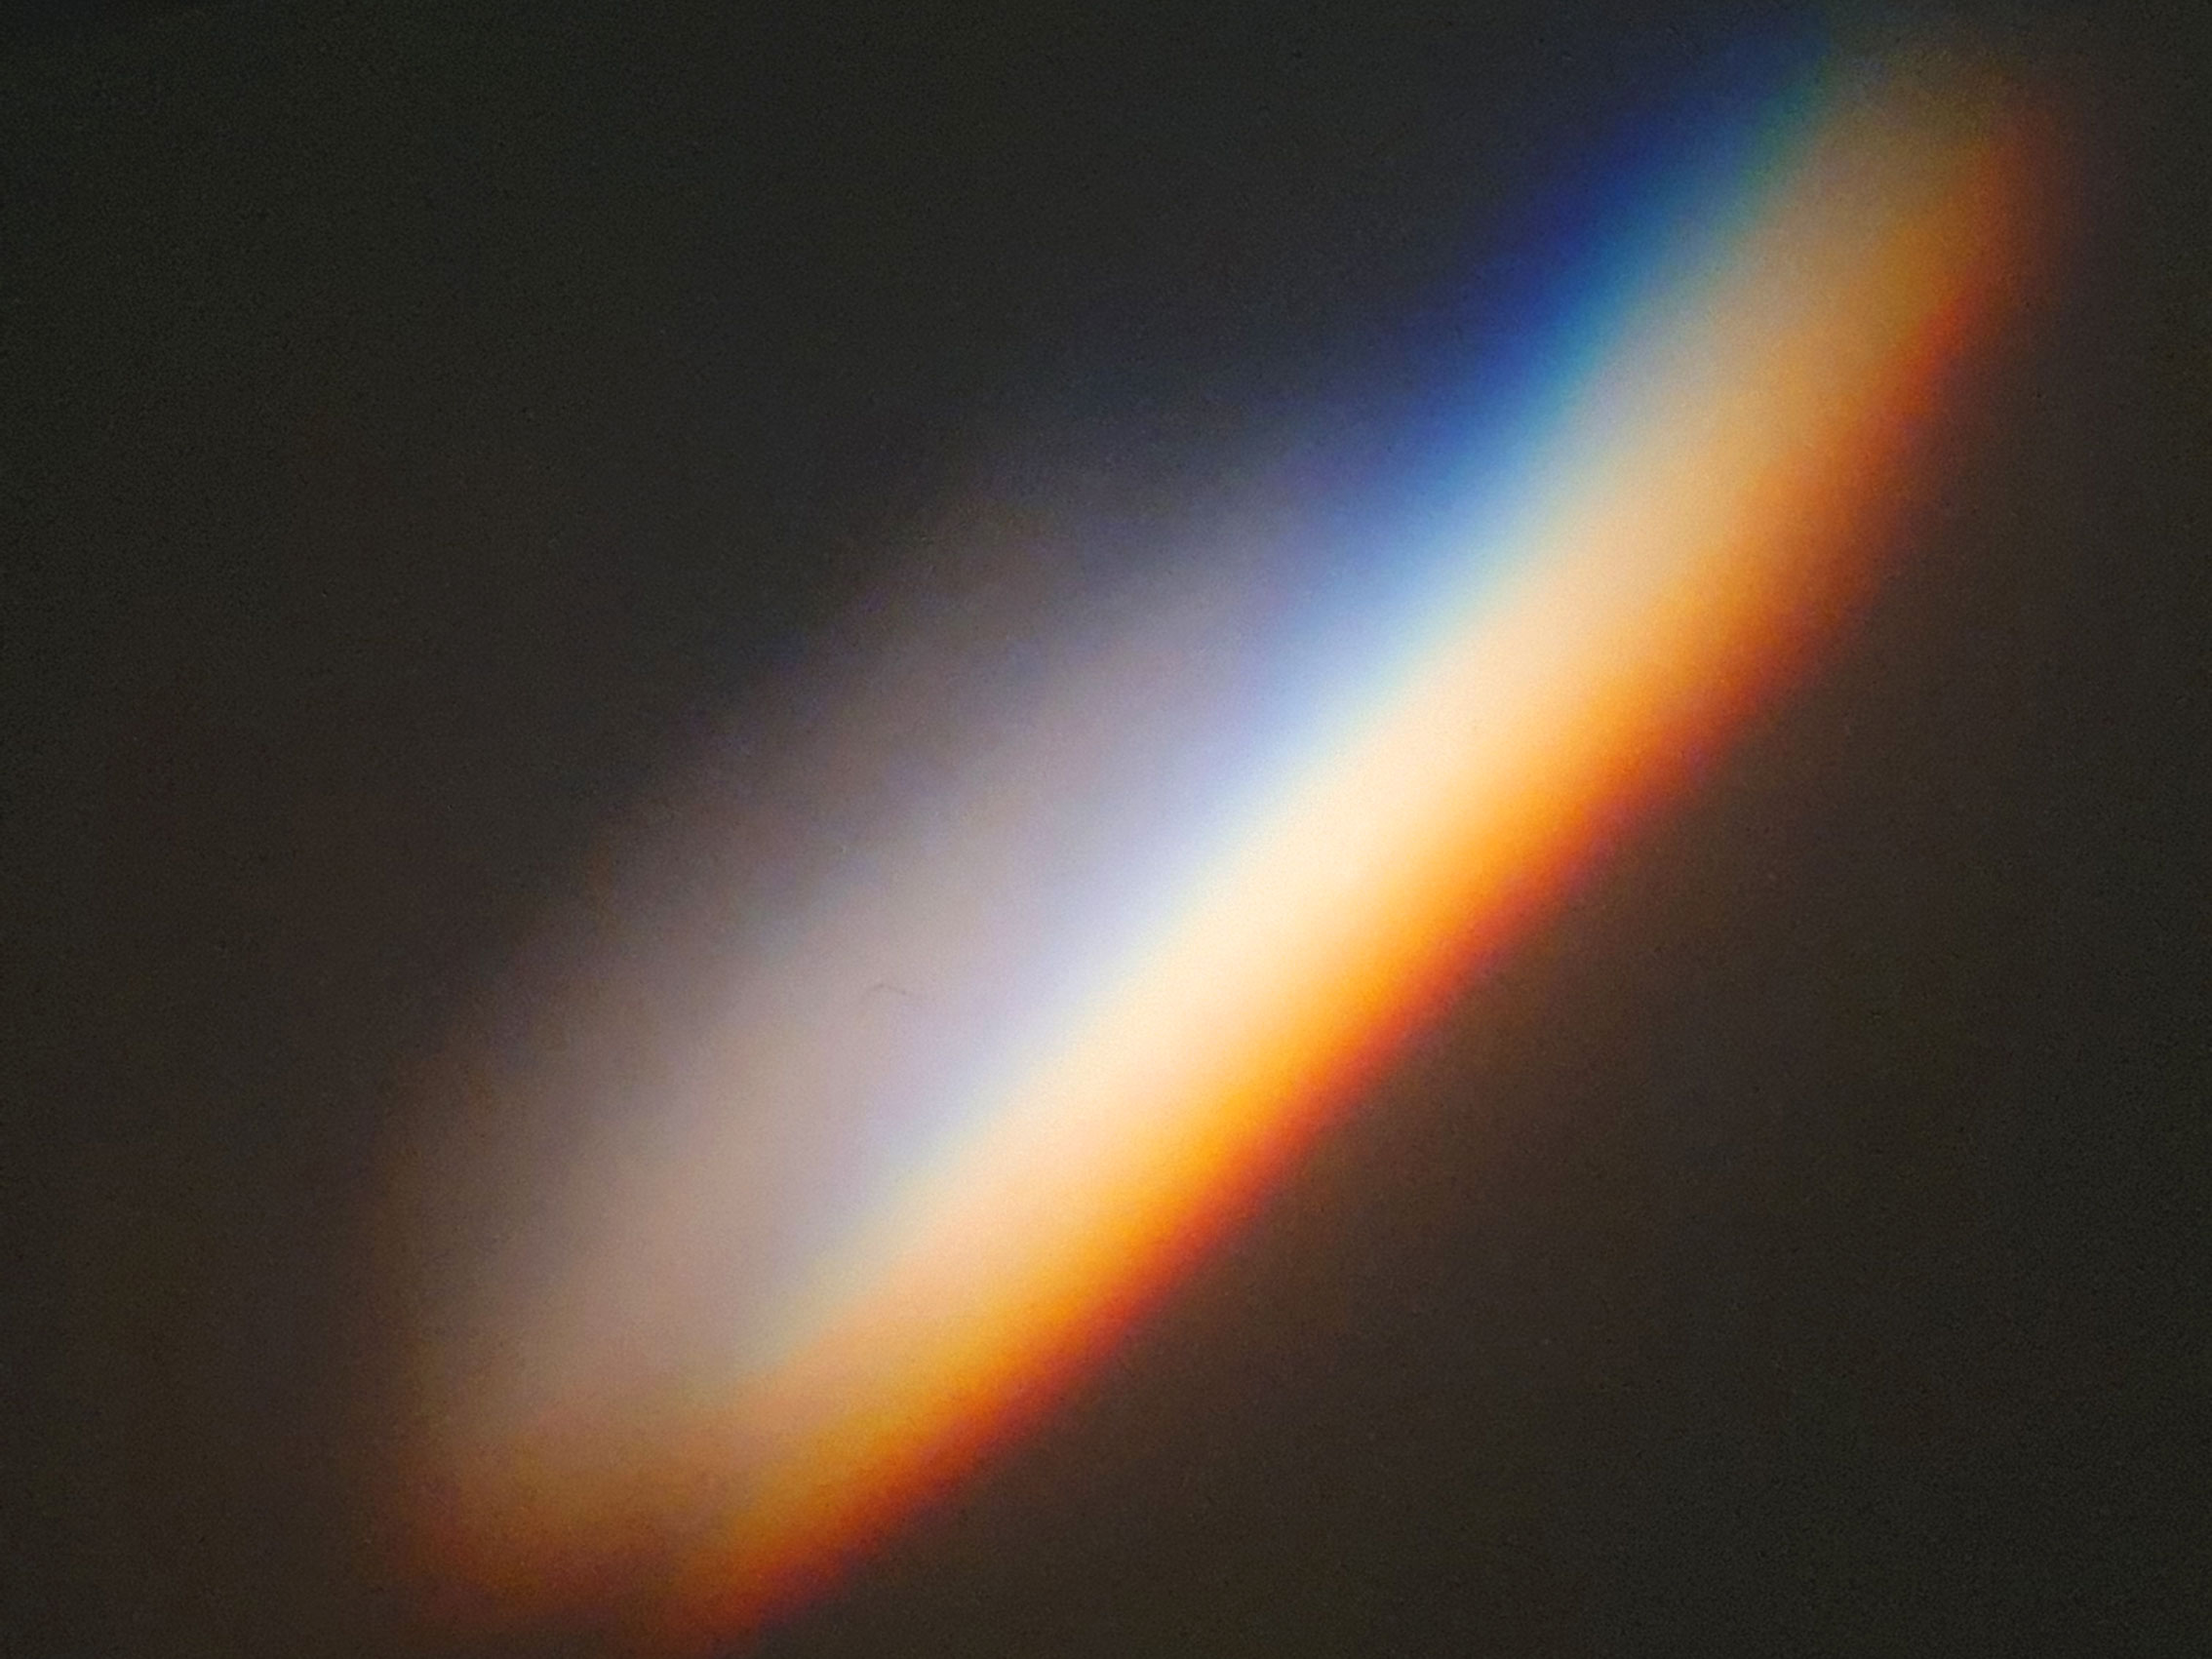
\includegraphics[width=0.6\linewidth]{nudes/komprimert/chr abb.jpg}
    \caption{Chromatische Aberration der Linse. }
    \label{fig:chrom_Abb}
\end{figure}

\section{Diskussion} %diskussion der Unsicherheiten und Ergebnisse und evtl. verlgeich mit Literatur ------------------------------
Dünne Linsen sind heutzutage überall zu finden. Jede Kamera, jedes Smartphone hat Linsen Verbaut. Durch diese lässt sich ein Bild auf einen Bildsensor darstellen. 
\\
\\
In dem Versuch ging es darum, die Brennweite $f$ einer Sammellinse und einer Zerstreuungslinse zu bestimmen. 
Wie man etwas schwer in den Abbildungen \ref{fig:aufbau Sammellinse} und \ref{fig:aufbau Zerstreuungslinse} erkennen kann, besitzen die Linsen eine Brennweite $f$ von 25 cm. 
Dieser Wert entspricht den Berechnungen, daher lässt sich bei diesen Teil auf eine fehlerfreie Durchführung schließen. 
\\
\\
Bei den Linsenfehlern gibt es einige interessante Beobachtungen. Selbst heute, bei modernster und präzisester Herstellung der Linsen finden sich dennoch Fehler vor. 
Eine gute Faustregel in der Fotografie ist es, je teurer die Optik im Kauf, desto besser wurde sie hergestellt, desto besser die Abbildungsqualität und geringere Linsenfehler. 
Wie man in Abbildung \ref{fig:chrom_Abb} erkennen kann, wird das Licht bei der Linse unterschiedlich stark gebrochen und es kommt zu Farbfehlern \cite{wiki1}. 
Moderne Kameras oder Bildbearbeitungsprogramme können diese Fehler aber korrigieren. 
Eine weitere Möglichkeit chromatische Aberration zu verhindern ist es Linsen mit unterschiedlicher Dispersion zu wählen, so dass die Wellenlängen wieder zusammengeführt werden \cite{wiki1}. 
\\
\\
Bei der Verzerrung handelt es sich um einen weiteren Linsenfehler. Dabei handelt es sich um eine Veränderung des Abbildungsmaßstabes \cite{wiki2}. 
Dieser Effekt tritt vorallem in Weitwinkligen Optiken auf. Moderne Bildbearbeitungsprogramme ermöglichen jedoch eine Korrektur des Fehlers. 

\section{Zusammenfassung} %klare, übersichtliche vollständige beantwortung der Aufgabenstellung ------------------------------
Hier nocheinmal die Ergebnise zusammengefasst. Hier werden nur die Mittelwerte der Ergebnisse dargestellt. 

\begin{itemize}
    \item Brennweite nach Laplace: $\bar{f} = (24.9 \pm 0.1) cm$
    \item Brennweite nach Bessel: $\bar{f} = (24.9 \pm 0.1) cm$
    \item Brennweite der Zerstreuungslinse: $\bar{f_s} = (-25.6 \pm 0.1)cm$
\end{itemize}

\printbibliography[heading=bibintoc]
\end{document}
